\documentclass[11pt,a4paper]{article}
\usepackage[margin=22mm]{geometry}
\usepackage[T1]{fontenc}
\usepackage{lmodern,tabularx,booktabs,hyperref,xcolor}
\setlength{\parindent}{0pt}\setlength{\parskip}{6pt}
\usepackage{graphicx,enumitem,microtype}
\setlist{itemsep=1pt,topsep=2pt,parsep=0pt}
\emergencystretch=1em
\hypersetup{colorlinks=true,linkcolor=black,urlcolor=blue!60!black}
\def\UrlBreaks{\do\/\do\_\do\-}
\newcommand{\field}[1]{\textbf{#1:}\ }
\newcommand{\code}[1]{\texttt{\detokenize{#1}}}
\newcolumntype{L}{>{\raggedright\arraybackslash}X}
\newcolumntype{P}[1]{>{\raggedright\arraybackslash}p{#1}}
\newcommand{\fig}[3]{\begin{center}\includegraphics[width=#1\linewidth]{#2}\\[2pt]{\small #3}\end{center}}
\begin{document}
\begin{center}\Large\textbf{23CSE455 Design Patterns}\\[4pt]\LARGE Case Study Report\end{center}

\field{Team} A5\par
\field{Case study} Healthcare Application using Laravel: ``Design Pattern Identification in a Laravel-Based Healthcare Management Application''\par
\field{Application} \code{esteham/hospital-management}. A public Laravel~12 application for patients, appointments, doctors, diagnostic tests, local billing fields and prescriptions.\par
\field{Date} 2026-10-10\par
\textbf{Submission repository:} \href{https://github.com/aswathymohan-amrita/23CSE455_DP_CaseStudy}{23CSE455\_DP\_CaseStudy} (team folder \code{A5/})\par
\textbf{Students}\par
\begin{tabularx}{\linewidth}{@{}lX@{}}\toprule
Roll number & Student name\\\midrule
AM.AL.U4AID23014 & Nemali Ashrith Reddy\\
AM.AL.U4AID23062 & Akshay Reddy Velugati\\
AM.SC.U4CSE23212 & B. Pravallika\\
AM.SC.U4CSE23022 & Daripineni Manogna\\\bottomrule
\end{tabularx}

\section{Application and architecture}
\field{Original source} \url{https://github.com/esteham/hospital-management}.
Baseline commit \code{1e7420e431771e3f5eec470d8a005e8255fa5fe8}, dated 17 November 2025.
The controllers and models examined for this report are copied in \path{data/code/}, together with \path{composer.json}. That folder is not a full clone. The rest of the application is the GitHub commit above. \code{vendor/} and \code{.env} are not included.\par

\field{Environment} PHP \^{}8.2 and Laravel 12 (\code{laravel/framework} \^{}12.0), read from \path{data/code/composer.json}.
The frontend is Vue~3 with Inertia. The database is MySQL through Eloquent.
Other confirmed packages are \code{barryvdh/laravel-dompdf} and \code{simplesoftwareio/simple-qrcode}.
Authentication uses Laravel Sanctum and Breeze.
Part~3 was run with Java 17, CPython 3.11.9, Node.js 22.14.0 and g++ (C++17) on Windows.\par

\field{Scope} We inspected the controllers and models for the six required modules:
\path{AppointmentController}, \path{Diagnostic/DiagnosticBookingController}, \path{Doctor/AppointmentController},
and the models \path{User}, \path{Appointment}, \path{Doctor}, \path{DiagnosticService}, \path{BookingDiagnostic}, \path{Prescription}, \path{PackageBooking} and \path{TestResult}.
There is no \code{app/Services}, \code{app/Repositories}, \code{app/Adapters} or \code{app/Observers} directory in this commit.\par

\field{Architecture} Figure~1 is the request path that exists today. A Vue and Inertia page reaches the Laravel router. The router calls a controller. The controller validates the request, applies the business rule, calls a framework facade when it needs mail or a PDF, and writes a row through an Eloquent model.
The same path covers the six modules. A patient is a user, a doctor is a linked profile, an appointment or a diagnostic booking is created in its controller, and a prescription is the medical record stored against that appointment.\par
\fig{0.92}{Part1/pattern_architecture/current_architecture.pdf}{Figure 1. Current architecture. The shaded bands are the layers that exist today.}

\field{Run instructions} The original application is run from a clone of the commit above, not from this folder: \code{composer install}, then \code{php artisan serve}.
The Part~3 programs are the programs we executed. Each language folder under \path{Part3/} has a README with the command. The printed results are in \path{data/test_result/}.

\section{Part 1 Pattern discovery}
\noindent\fbox{\parbox{\dimexpr\linewidth-2\fboxsep-2\fboxrule}{\small
\textbf{What the source actually uses}\\[2pt]
\textbf{Active Record:} an Eloquent model is the table. \code{Appointment::create} writes the row.\\
\textbf{Facade (framework only):} controllers call Laravel facades (\code{Auth}, \code{Mail}, \code{Validator}, \code{DB}, \code{Pdf}). There is no application facade class.\\
\textbf{Not found:} Adapter, Proxy, Strategy, Repository, Observer, and a service layer.}}
\medskip

\field{Method} We opened the files in \path{data/code/}. A pattern was recorded only when a class relationship in those files supports it. A Laravel built-in was labelled as framework code. A name that appears only in a README was not counted.
The two types that met that test are Active Record, because the Eloquent model is the table row, and Facade, because the controllers call Laravel's \code{Mail}, \code{Pdf}, \code{Auth}, \code{Validator}, and \code{DB}. The payment list and the mail call inside \code{storePrescription} were read and were not counted as Strategy or Observer.\par

\subsection{Totals at the baseline}
\field{Confirmed pattern types} 2: Active Record and Facade.\par
\field{Facade scope} Framework only. No custom facade was found under \code{app/}.\par
\field{Not identified} Adapter, Proxy, Repository, Service layer, Strategy and Observer.\par
\field{Observation scope} The files listed in Section~1, at commit \code{1e7420e}.

{\small\begin{tabularx}{\linewidth}{@{}P{42mm}L@{}}\toprule
Rejected candidate & Reason\\\midrule
Adapter & No class translates an external payload into the application's fields.\\
Proxy & No surrogate stands in front of a model or a remote call.\\
Strategy & \code{payment\_method} is the string list \code{cash}, \code{card}, \code{online}. It is not a family of classes.\\
Repository & Queries are written in the controllers.\\
Service layer & There is no \code{app/Services} directory. \code{DiagnosticService} is an Eloquent model.\\
Observer & \code{Mail::to} is called inside \code{storePrescription}, not from a model observer.\\
Application Facade & The \code{use Facade} lines are Laravel's own facades.\\\bottomrule
\end{tabularx}}

\subsection{Pattern inventory}
\begin{tabularx}{\linewidth}{@{}lXll@{}}\toprule
Pattern type & Instance names & Instances & Where\\\midrule
Active Record & Appointment row, Diagnostic payment flags, Patient and doctor identity & 3 & Application\\
Facade & Prescription mail and PDF, Controller facades & 2 & Framework only\\\bottomrule
\end{tabularx}

Data files: \path{Part1/patterns.csv} and \path{Part1/Pattern_count.csv}.

\subsection{One record for each pattern instance}

\subsubsection*{Record 1: Appointment row}
\field{Instance name} Appointment row\par
\field{Pattern type and category} Active Record. The model is the persistence object.\par
\field{Purpose} \code{AppointmentController::store} checks the doctor's daily capacity and then inserts the booking.\par
\textbf{Participant mapping}\par
{\small\begin{tabularx}{\linewidth}{@{}P{28mm}LX@{}}\toprule
Pattern role & Actual class and function & File and line range\\\midrule
Model & \code{Appointment} & \path{data/code/app/Models/Appointment.php:8-39}\\
Create & \code{Appointment::create} inside \code{store} & \path{data/code/app/Http/Controllers/AppointmentController.php:56-121}\\
Relation & \code{Appointment::doctor}, \code{Appointment::prescriptions} & \path{data/code/app/Models/Appointment.php:26-39}\\\bottomrule
\end{tabularx}}
\field{Evidence} The capacity check and the insert are in the same controller method. \code{Schedule} is queried with \code{whereJsonContains} before the row is created. Mail is sent from that method through the \code{Mail} facade (lines 111 and 121).\par

\subsubsection*{Record 2: Diagnostic payment flags}
\field{Instance name} Diagnostic payment flags\par
\field{Pattern type and category} Active Record, with a framework Facade for validation and PDF.\par
\field{Purpose} A diagnostic booking is stored locally. No payment gateway is called.\par
\textbf{Participant mapping}\par
{\small\begin{tabularx}{\linewidth}{@{}P{28mm}LX@{}}\toprule
Pattern role & Actual class and function & File and line range\\\midrule
Model & \code{BookingDiagnostic} & \path{data/code/app/Models/BookingDiagnostic.php:7-59}\\
Validation & \code{payment\_method} in cash, card, online & \path{DiagnosticBookingController.php:55}\\
Facade & \code{Validator}, \code{Auth}, \code{Pdf} & lines 10--14 and 134 of the same controller\\\bottomrule
\end{tabularx}}
\field{Evidence} \code{store} sets \code{payment\_status} to \code{pending} and calls \code{BookingDiagnostic::create}. \code{composer.json} does not require Stripe, PayPal or any other payment package. Package bookings are a different table, with \code{payment\_type}, \code{amount\_paid} and \code{total\_amount} (\path{data/code/app/Models/PackageBooking.php}).\par

\subsubsection*{Record 3: Prescription mail and PDF}
\field{Instance name} Prescription mail and PDF\par
\field{Pattern type and category} Framework Facade, used from a fat controller.\par
\field{Purpose} The doctor who owns the appointment writes \code{prescription\_text} and emails a PDF.\par
\textbf{Participant mapping}\par
{\small\begin{tabularx}{\linewidth}{@{}P{28mm}LX@{}}\toprule
Pattern role & Actual class and function & File and line range\\\midrule
Model & \code{Prescription} & \path{data/code/app/Models/Prescription.php:7-18}\\
Controller & \code{storePrescription} & \path{data/code/app/Http/Controllers/Doctor/AppointmentController.php:71-94}\\
Facades & \code{Pdf::loadView}, \code{Mail::to} & lines 90 and 94\\\bottomrule
\end{tabularx}}
\field{Evidence} The ownership check, the insert, the PDF and the mail send are one method. The mail send is inside a try/catch in that method. This is not an Observer.\par

\subsubsection*{Record 4: Patient and doctor identity}
\field{Instance name} Patient and doctor identity\par
\field{Pattern type and category} Active Record.\par
\field{Purpose} A patient is a \code{User} with a role. A doctor profile is a \code{Doctor} row that belongs to that user. There is no \code{Patient} model.\par
\textbf{Participant mapping}\par
{\small\begin{tabularx}{\linewidth}{@{}P{28mm}LX@{}}\toprule
Pattern role & Actual class and function & File and line range\\\midrule
User & \code{User::doctor}, \code{User::staff} & \path{data/code/app/Models/User.php:15-32}\\
Doctor & \code{Doctor::user}, \code{Doctor::schedules} & \path{data/code/app/Models/Doctor.php:8-16}\\\bottomrule
\end{tabularx}}
\field{Evidence} Appointment rows also store \code{first\_name}, \code{last\_name}, \code{email} and \code{phone} on the booking itself, so a booking does not require a user foreign key.\par

\section{Part 2 Evolution study}
Part~2 does not change commit \code{1e7420e}. It records what the design would have to become for three external systems. Epic, Quest Diagnostics, Stripe and PayPal are examples. They are not integrations in the repository. Dashed boxes in Figure~2 are proposed.
The laboratory and the health record each need a class that translates an outside payload, so both use Adapter. Billing needs two providers behind one call, so that change uses Strategy. In that design the controller still validates the HTTP request, and the service makes the outside call.

\begin{tabularx}{\linewidth}{@{}P{28mm}LL@{}}\toprule
Integration & As coded & Proposed\\\midrule
Laboratory & \code{DiagnosticBookingController} creates \code{BookingDiagnostic} & \code{LaboratoryIntegrationService}, \code{LaboratoryIntegrationInterface}, \code{QuestDiagnosticsAdapter}\\
Billing & Controller stores \code{payment\_method} and \code{payment\_status} & \code{BillingService}, \code{PaymentStrategy}, \code{StripePayment}, \code{PayPalPayment}\\
Patient data & Controller reads \code{User}, \code{Appointment}, \code{Prescription} & \code{PatientDataService}, \code{EHRProvider}, \code{EpicEHRAdapter}, \code{EpicFHIRApi}\\\bottomrule
\end{tabularx}

\begin{tabularx}{\linewidth}{@{}P{24mm}LX@{}}\toprule
Pattern & Job & Phase\\\midrule
Adapter & Translates a nested FHIR sample into first name, last name and phone. A laboratory adapter does the same job for a vendor payload. & Part~3 implements the EHR adapter. The Quest adapter stays a proposal.\\
Strategy & Swaps Stripe and PayPal behind one payment call. The context has no provider branch. & Part~3\\
Proxy & A cache proxy would return a stored EHR copy when it has one. & Proposal only\\
Service layer & Moves the orchestration out of the controller. & Described with the two Part~3 patterns\\
Facade & The existing Laravel facades stay as they are. & Unchanged\\\bottomrule
\end{tabularx}

\field{Naming rule} The proposed laboratory service is \code{LaboratoryIntegrationService}. The name \code{DiagnosticService} is already the catalogue model (\path{data/code/app/Models/DiagnosticService.php:7}).\par

\fig{0.98}{Part2/diagrams/evolved_architecture.pdf}{Figure 2. Evolved architecture. The left band is the application we inspected. The dashed band is proposed.}
\fig{0.88}{Part2/diagrams/adapter_uml.pdf}{Figure 3. Adapter class diagram for the proposed EHR integration.}
\fig{0.88}{Part2/diagrams/strategy_uml.pdf}{Figure 4. Strategy class diagram for the proposed billing providers.}

\field{Refactoring} In the original design the business rule stays in the controller. After the proposed refactoring the controller still validates HTTP input. It does not parse FHIR and it does not switch on a provider name. This refactoring has not been applied to the upstream repository. The notes for the three changes are in \path{Part2/changes/Change1/}, \path{Change2/} and \path{Change3/}. The proposed PHP roles are in \path{Part2/code/}.

\section{Part 3 Cross-language implementations}
The two patterns written in Part~3 are Adapter and Strategy. The four languages are Java, Python, JavaScript and C++. The original application remains Laravel and PHP. None of the programs opens a network connection.
Each program builds the concrete adapter or strategy at the start and passes it into the client through the constructor. All four languages use patient \code{PT-98765} and the references \code{DX-1001} and \code{DX-1002}, and the files in \path{data/test_result/} are the output of those runs.

{\small\begin{tabularx}{\linewidth}{@{}llL@{}}\toprule
Language & Role & Class\\\midrule
Java, Python, C++ & Adapter target & \code{EHRProvider}\\
JavaScript & Adapter target & the same method names, with no compile-time interface\\
All four & Adapter client & \code{PatientDataService}\\
All four & Strategy context & \code{BillingService}\\
All four & Concrete strategies & \code{StripePayment} and \code{PayPalPayment}\\\bottomrule
\end{tabularx}}

{\small\begin{tabularx}{\linewidth}{@{}lP{34mm}L@{}}\toprule
Language & Version used & Test command\\\midrule
Java & Java 17 & \code{javac AdapterDemo.java} then \code{java AdapterDemo}\\
Python & CPython 3.11.9 & \code{python adapter_demo.py}\\
JavaScript & Node.js 22.14.0 & \code{node adapterDemo.js}\\
C++ & g++, C++17 & \code{g++ -std=c++17 adapter_demo.cpp -o adapter_demo} then run it\\\bottomrule
\end{tabularx}}

The Strategy commands are the same, with the file names in \path{Part3/strategy/}.\par

\field{Actual results} The adapter programs print \code{first\_name} John, \code{last\_name} Smith and phone \code{555-1234} for patient \code{PT-98765}. The strategy programs print provider \code{stripe} for reference \code{DX-1001} and provider \code{paypal} for reference \code{DX-1002}. The captured output is in \path{data/test_result/}. The JavaScript and C++ adapter programs exit with code 1 if those three patient fields are wrong. The JavaScript and C++ strategy programs exit with code 1 if the provider name is wrong.\par

\field{Comparison}
\begin{itemize}
\item The client receives the interface through its constructor in every language. The concrete adapter or strategy is built at the start of the program.
\item Java and C++ state the contract as an interface or an abstract class. Python uses an abstract base class. JavaScript uses the same method names without a compile-time interface.
\item Python spells the adapter method \code{get\_patient\_record}. The other three languages spell it \code{getPatientRecord}.
\item The comparison files are \path{Part3/adapter/pattern_crosslanguage.csv} and \path{Part3/strategy/pattern_crosslanguage.csv}. The source-location column is the non-blank line count of each program. Cyclomatic complexity and process time were not measured, so those two columns say ``not measured''.
\end{itemize}

\section{LLM evidence}
An LLM drafted explanations and the first versions of the four-language programs. A claim about the repository was kept only when the file in \path{data/code/} supported it. During the investigation the LLM could not read the GitHub tree, so the module map was rebuilt from the files we opened. The working thread is \url{https://share.gemini.google/zjKon9gmTNO8}.

{\small\begin{tabularx}{\linewidth}{@{}P{32mm}LL@{}}\toprule
Task & What was drafted & What was kept after checking\\\midrule
Choose the application & Three public Laravel repositories & The empty skeleton was dropped. This report uses \code{esteham/hospital-management}.\\
Name existing patterns & Several GoF names, including Adapter & Adapter, Proxy, Strategy, Repository, Observer and a service layer are marked not identified.\\
Evolve the design & Adapter, Strategy, Proxy and services & Billing is Strategy. The proxy and the Quest adapter stay proposals.\\
Laboratory service name & The first draft reused \code{DiagnosticService} & Renamed to \code{LaboratoryIntegrationService}.\\
Part 3 languages & PHP and TypeScript were drafted first & The submitted languages are Java, Python, JavaScript and C++, as required.\\\bottomrule
\end{tabularx}}

The check against the Gemini thread is \path{Part1/llm/verification.md}. The record files are \path{Part1/llm.csv}, \path{Part2/llm.csv}, \path{Part3/adapter/llm/llm.csv} and \path{Part3/strategy/llm/llm.csv}.

\section{Contributions}
The four members divided the case study into equal parts.

{\small\begin{tabularx}{\linewidth}{@{}P{42mm}L@{}}\toprule
Student & Work\\\midrule
Nemali Ashrith Reddy & Part 1. Inspection of the hospital modules, the pattern inventory, and the current architecture.\\
Akshay Reddy Velugati & Part 2. The laboratory, billing, and patient-data evolution, with the evolved architecture and the UML diagrams.\\
B. Pravallika & Part 3, Adapter. The same EHR adapter in Java, Python, JavaScript, and C++, and the captured adapter output.\\
Daripineni Manogna & Part 3, Strategy. The same payment strategy in Java, Python, JavaScript, and C++, and the captured strategy output.\\\bottomrule
\end{tabularx}}

\section{Screenshot}
\begin{center}
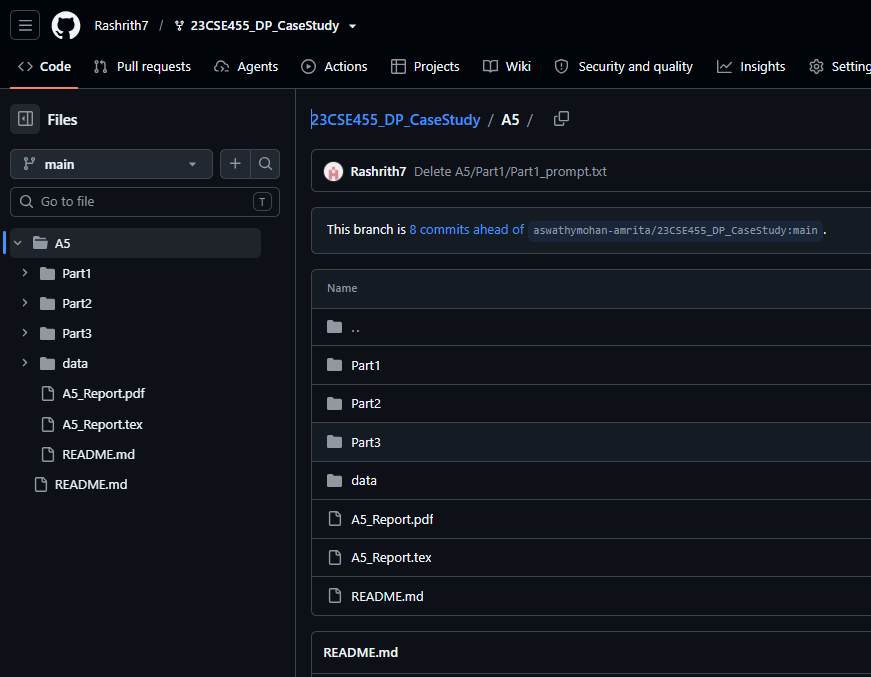
\includegraphics[width=\linewidth]{screenshot.png}
\end{center}

\section{Conclusion}
\code{esteham/hospital-management} at commit \code{1e7420e} implements the six healthcare areas with Eloquent models and with controllers that hold the business rules. The patterns supported by that source are Active Record and Laravel's own facades. Adapter, Strategy, Proxy, Repository, Observer and a service layer were not found.

Adapter is the translation point if an electronic health record is added. Strategy is the switch if a real payment provider is added. Those two patterns are implemented in Java, Python, JavaScript and C++. The laboratory adapter and the cache proxy remain proposals, so this report does not describe code that was not written.

\begin{thebibliography}{9}
\bibitem{hms} Esteham H. Zihad Ansari. Hospital Management. \url{https://github.com/esteham/hospital-management}.
\bibitem{gof} E.~Gamma, R.~Helm, R.~Johnson and J.~Vlissides. \emph{Design Patterns: Elements of Reusable Object-Oriented Software}. Addison-Wesley, 1994.
\bibitem{laravel} Laravel 12 documentation, facades and Eloquent. \url{https://laravel.com/docs/12.x}.
\end{thebibliography}
\end{document}
